%%%%%%%%%%%%%%%%%%%%%%%%%%%%%%%%%%%%%%%%%%%%%%%%%%%
\begin{frame}
  \begin{center}
    {\Large RNN with TensorFlow}
    
  \end{center}
\end{frame}

%%%%%%%%%%%%%%%%%%%%%%%%%%%%%%%%%%%%%%%%%%%%%%%%%%%
\begin{frame}[fragile] \frametitle{Sample Program: Echo-RNN}
A simple Echo-RNN remembers the input data and then echoes it after a few time-steps. 

Setup:

\begin{lstlisting}
import numpy as np
import tensorflow as tf
import matplotlib.pyplot as plt

num_epochs = 100
total_series_length = 50000
truncated_backprop_length = 15
state_size = 4
num_classes = 2
echo_step = 3
batch_size = 5
num_batches = total_series_length//batch_size//truncated_backprop_length
\end{lstlisting}

\end{frame}

%%%%%%%%%%%%%%%%%%%%%%%%%%%%%%%%%%%%%%%%%%%%%%%%%%%
\begin{frame}[fragile] \frametitle{Sample Program: Echo-RNN}

The input is basically a random binary vector. The output will be the ``echo'' of the input, shifted echo\_step steps to the right.

Generate data:
\begin{lstlisting}
def generateData():
    x = np.array(np.random.choice(2, total_series_length, p=[0.5, 0.5]))
    y = np.roll(x, echo_step)
    y[0:echo_step] = 0

    x = x.reshape((batch_size, -1))  # The first index changing slowest, subseries as rows
    y = y.reshape((batch_size, -1))

    return (x, y)
\end{lstlisting}
The reshaping of the data into a matrix with batch\_size rows.
\end{frame}


%%%%%%%%%%%%%%%%%%%%%%%%%%%%%%%%%%%%%%%%%%%%%%%%%%%
\begin{frame}[fragile] \frametitle{Sample Program: Building Graph}

\begin{itemize}
\item On each run the batch data is fed to the placeholders
\item These are ``starting nodes'' of the computational graph
\item  RNN init-state is supplied in a placeholder, which is saved from the output of the previous run. 
\end{itemize}

\begin{lstlisting}
batchX_placeholder = tf.placeholder(tf.float32, [batch_size, truncated_backprop_length])
batchY_placeholder = tf.placeholder(tf.int32, [batch_size, truncated_backprop_length])

init_state = tf.placeholder(tf.float32, [batch_size, state_size])
\end{lstlisting}
 
\end{frame}

%%%%%%%%%%%%%%%%%%%%%%%%%%%%%%%%%%%%%%%%%%%%%%%%%%%
\begin{frame}[fragile] \frametitle{Sample Program: Building Graph}

The weights and biases of the network are declared as TensorFlow variables

\begin{lstlisting}
W = tf.Variable(np.random.rand(state_size+1, state_size), dtype=tf.float32)
b = tf.Variable(np.zeros((1,state_size)), dtype=tf.float32)

W2 = tf.Variable(np.random.rand(state_size, num_classes),dtype=tf.float32)
b2 = tf.Variable(np.zeros((1,num_classes)), dtype=tf.float32)
\end{lstlisting}
 
\end{frame}


%%%%%%%%%%%%%%%%%%%%%%%%%%%%%%%%%%%%%%%%%%%%%%%%%%%
\begin{frame}[fragile] \frametitle{Sample Program: Training}

Want to do is calculate the sum of two affine transforms $current\_input * Wa + current\_state * Wb$ in the figure below. By concatenating those two tensors you will only use one matrix multiplication.

\begin{lstlisting}
# Forward pass
current_state = init_state
states_series = []
for current_input in inputs_series:
    current_input = tf.reshape(current_input, [batch_size, 1])
    input_and_state_concatenated = tf.concat(1, [current_input, current_state])  # Increasing number of columns

    next_state = tf.tanh(tf.matmul(input_and_state_concatenated, W) + b)  # Broadcasted addition
    states_series.append(next_state)
current_state = next_state
\end{lstlisting}
 \end{frame}



%%%%%%%%%%%%%%%%%%%%%%%%%%%%%%%%%%%%%%%%%%%%%%%%%%%
\begin{frame}[fragile] \frametitle{Training}

\begin{center}
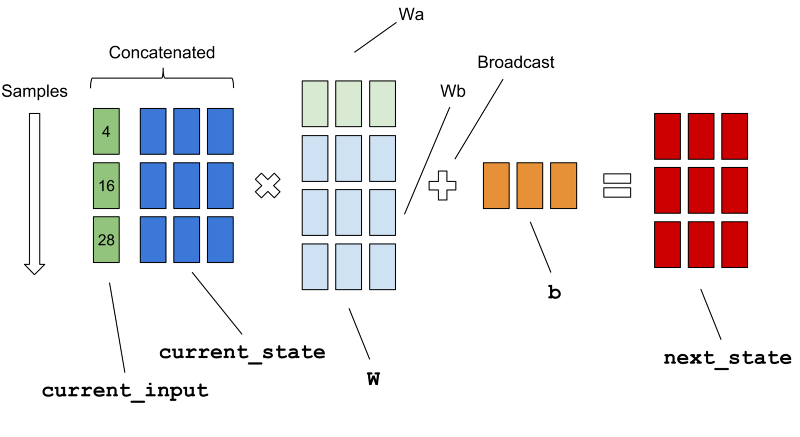
\includegraphics[width=\linewidth,keepaspectratio]{ericrnnwts}
\end{center}
\end{frame}

%%%%%%%%%%%%%%%%%%%%%%%%%%%%%%%%%%%%%%%%%%%%%%%%%%%
\begin{frame}[fragile] \frametitle{Sample Program: Calculating loss}
Logits is of shape $[batch\_size, num\_classes]$ and labels of shape $[batch\_size]$

\begin{lstlisting}
logits_series = [tf.matmul(state, W2) + b2 for state in states_series] #Broadcasted addition
predictions_series = [tf.nn.softmax(logits) for logits in logits_series]

losses = [tf.nn.sparse_softmax_cross_entropy_with_logits(logits, labels) for logits, labels in zip(logits_series,labels_series)]
total_loss = tf.reduce_mean(losses)

train_step = tf.train.AdagradOptimizer(0.3).minimize(total_loss)
\end{lstlisting}
 \end{frame}

%%%%%%%%%%%%%%%%%%%%%%%%%%%%%%%%%%%%%%%%%%%%%%%%%%%
\begin{frame}[fragile] \frametitle{Sample Program: Running a training session}

\begin{lstlisting}
with tf.Session() as sess:
    sess.run(tf.initialize_all_variables())
    loss_list = []

    for epoch_idx in range(num_epochs):
        x,y = generateData()
        _current_state = np.zeros((batch_size, state_size))
        
        for batch_idx in range(num_batches):
            start_idx = batch_idx * truncated_backprop_length
            end_idx = start_idx + truncated_backprop_length

            batchX = x[:,start_idx:end_idx]
            batchY = y[:,start_idx:end_idx]

            _total_loss, _train_step, _current_state, _predictions_series = sess.run(
                [total_loss, train_step, current_state, predictions_series],
                feed_dict={batchX_placeholder:batchX,batchY_placeholder:batchY,init_state:_current_state})

            loss_list.append(_total_loss)

            if batch_idx\%100 == 0:
                print("Step",batch_idx, "Loss", _total_loss)
                plot(loss_list, _predictions_series, batchX, batchY)

\end{lstlisting}
\end{frame}


%%%%%%%%%%%%%%%%%%%%%%%%%%%%%%%%%%%%%%%%%%%%%%%%%%%
\begin{frame}[fragile] \frametitle{Sample Program: Using RNN Cell}
The forward pass code can be replaced by

\begin{lstlisting}
# Unpack columns
inputs_series = tf.split(1, truncated_backprop_length, batchX_placeholder)
labels_series = tf.unpack(batchY_placeholder, axis=1)

# Forward passes
cell = tf.nn.rnn_cell.BasicRNNCell(state_size)
states_series, current_state = tf.nn.rnn(cell, inputs_series, init_state)
\end{lstlisting}
You may also remove the weight- and bias matrices $W$ and $b$ declared earlier. The inner workings of the RNN are now hidden.
\end{frame}


%%%%%%%%%%%%%%%%%%%%%%%%%%%%%%%%%%%%%%%%%%%%%%%%%%%
\begin{frame}[fragile] \frametitle{Feed-forward Neural Network in Query Classification}
To classify a specific sentence query into some pre-defined categories. Steps:

\begin{itemize}
\item Tokenization of a query-sentence. Convert to some W2V representation
\item Extract regular expression features from the corresponding sentences, like POS tags, etc. Convert to One-hot encoding
\item Feed these vectors to Deep Learning model
\end{itemize}
\begin{center}
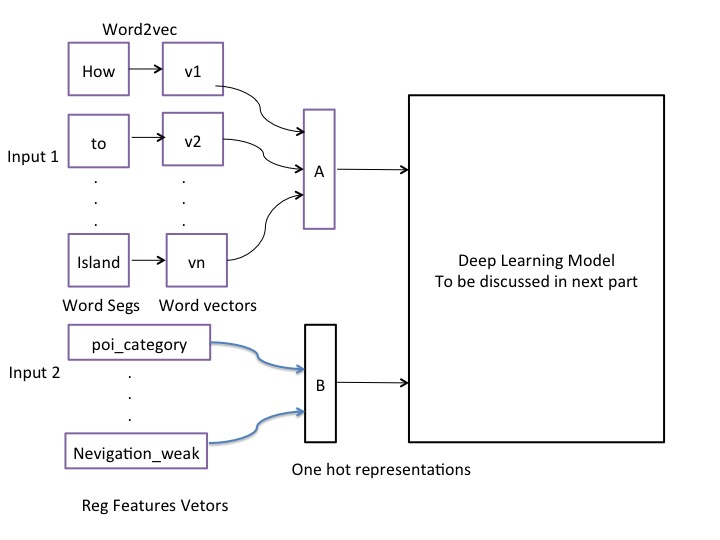
\includegraphics[width=0.4\linewidth,keepaspectratio]{qryinputs}
\end{center}
Each deep learning model has different way of feeding input.
\end{frame}


%%%%%%%%%%%%%%%%%%%%%%%%%%%%%%%%%%%%%%%%%%%%%%%%%%%
\begin{frame}[fragile] \frametitle{Feed-forward Neural Network in Query Classification}
\begin{itemize}
\item The input fed into a Feed-forward Neural Network is in a parallel manner, i.e. one query's information as one input. 
\item Word vectors of all words in sentence are combined by averaging.
\end{itemize}
\begin{center}
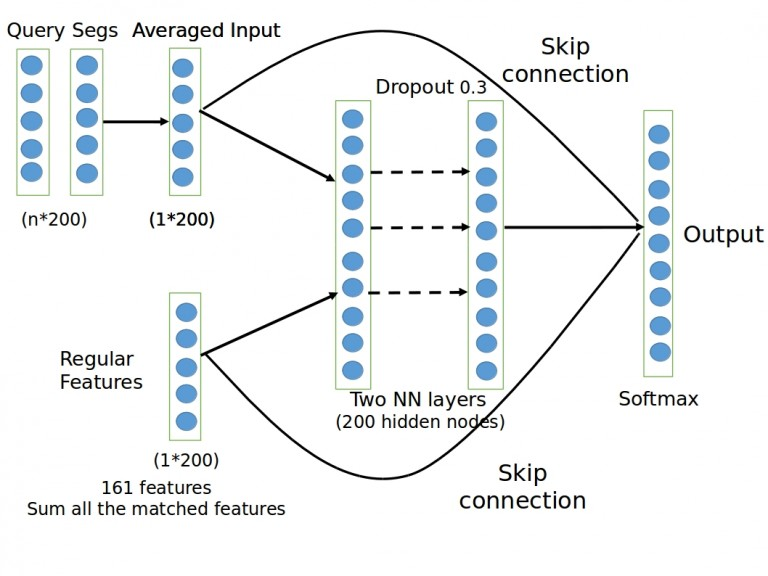
\includegraphics[width=0.6\linewidth,keepaspectratio]{qrymodel}
\end{center}
\end{frame}


%%%%%%%%%%%%%%%%%%%%%%%%%%%%%%%%%%%%%%%%%%%%%%%%%%%
\begin{frame}[fragile] \frametitle{Feed-forward Neural Network in Query Classification}
\begin{itemize}
\item Two skip connections go from inputs to output directly
\item Mainly for learning the linear relations between input and output, as most have strong linear relations towards the output.
\end{itemize}
Problem: Due to averaging, the order and context are lost. Need to look at other models.
\end{frame}




%%%%%%%%%%%%%%%%%%%%%%%%%%%%%%%%%%%%%%%%%%%%%%%%%%%
\begin{frame}[fragile] \frametitle{Recurrent Neural Network in Query Classification}
\begin{itemize}
\item LTSM overcomes the disadvantage that gradient vanishing in conventional RNN
\item Due to forget gate, LSTM is better for long lags between inputs.
\end{itemize}
\begin{center}
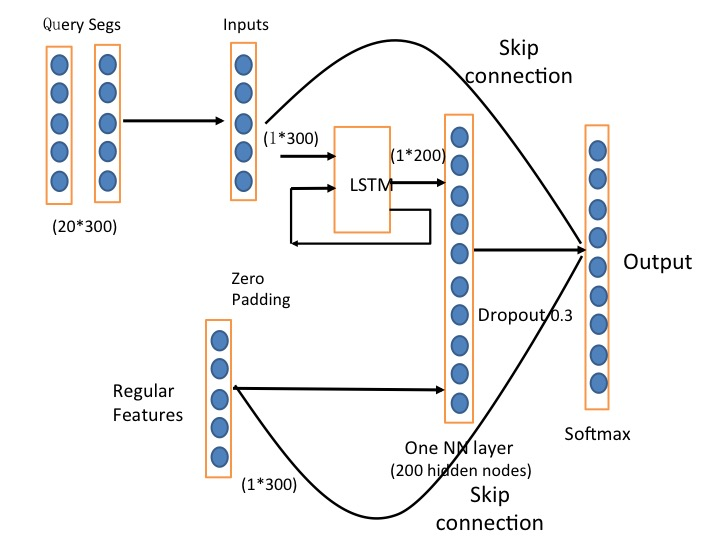
\includegraphics[width=0.6\linewidth,keepaspectratio]{qrylstm}
\end{center}
\end{frame}


%%%%%%%%%%%%%%%%%%%%%%%%%%%%%%%%%%%%%%%%%%%%%%%%%%%
\begin{frame}[fragile] \frametitle{Recurrent Neural Network in Query Classification}
\begin{itemize}
\item LSTM is a model taking sequential inputs, word vectors one by one
\item Also keeps the memory of given number of words (say, a full sentence)
\end{itemize}
\end{frame}


%%%%%%%%%%%%%%%%%%%%%%%%%%%%%%%%%%%%%%%%%%%%%%%%%%%
\begin{frame}[fragile] \frametitle{Input preparation for LSTM}
\begin{itemize}
\item Query sentances have variable lengths
\item In Tensorflow, however, only fixed size of number of input query segment is accepted. 
\item Paddings are needed for shorter sentences, and cut off is applied through longer ones. 
\item In the example above, 20 word vectors are limited for one query as an input.
\end{itemize}
\end{frame}


%%%%%%%%%%%%%%%%%%%%%%%%%%%%%%%%%%%%%%%%%%%%%%%%%%%
\begin{frame}[fragile] \frametitle{Input preparation for LSTM}
\begin{lstlisting}
#Create layers in Tensorflow
        lstm= tf.nn.rnn_cell.BasicLSTMCell(200, forget_bias=1.0)
        state=tf.zeros([1,200])
        num_steps=20
# the input x_in is a list of 20 1*300 vectors
        output_lstm, state = rnn.rnn(lstm, x_in, dtype=tf.float32)
# get the last element of a list, i.e the output from lstm to be fed into the dense NN
        output_lstm=output_lstm[-1]
        lin_h=tf.matmul(output_lstm,self.hiddenLayer.W)+self.hiddenLayer.b
\end{lstlisting}
\end{frame}


%%%%%%%%%%%%%%%%%%%%%%%%%%%%%%%%%%%%%%%%%%%%%%%%%%%
\begin{frame}[fragile] \frametitle{LSTM Model}
\begin{lstlisting}
        reg_h = tf.reduce_sum(tf.gather(self.reg_lookup_table, self.reg_x), 0)
        h = self.activation(lin_h + tf.cast(reg_h,tf.float32))
        lin_output_pre = tf.matmul(h, self.outputLayer.W) + self.outputLayer.b
        lin_output = tf.nn.dropout(lin_output_pre, keep_prob=0.6)
        reg_output = tf.reduce_sum(tf.gather(self.skip_layer_re.W, self.reg_x), 0) + self.skip_layer_re.b
        ae_output = tf.matmul(x_in[-1], self.skip_layer_ae.W) + self.skip_layer_ae.b 
        ae_output = tf.nn.dropout(ae_output, keep_prob=0.5)
        output = tf.nn.softmax(lin_output + ae_output + reg_output)
\end{lstlisting}

All the ``hidden layer'', ``skip layer'' etc. are the ``Layer'' object, and the initialization of ``W'' and ``b'' are is also implemented in ``Layer'' class.
\end{frame}


%%%%%%%%%%%%%%%%%%%%%%%%%%%%%%%%%%%%%%%%%%%%%%%%%%%
\begin{frame}[fragile] \frametitle{TensorFlow: GRU}
\begin{itemize}
\item Ready GRU cell network available
\item Variable length sequences can be handled by dynamic rnn
\end{itemize}
\begin{center}
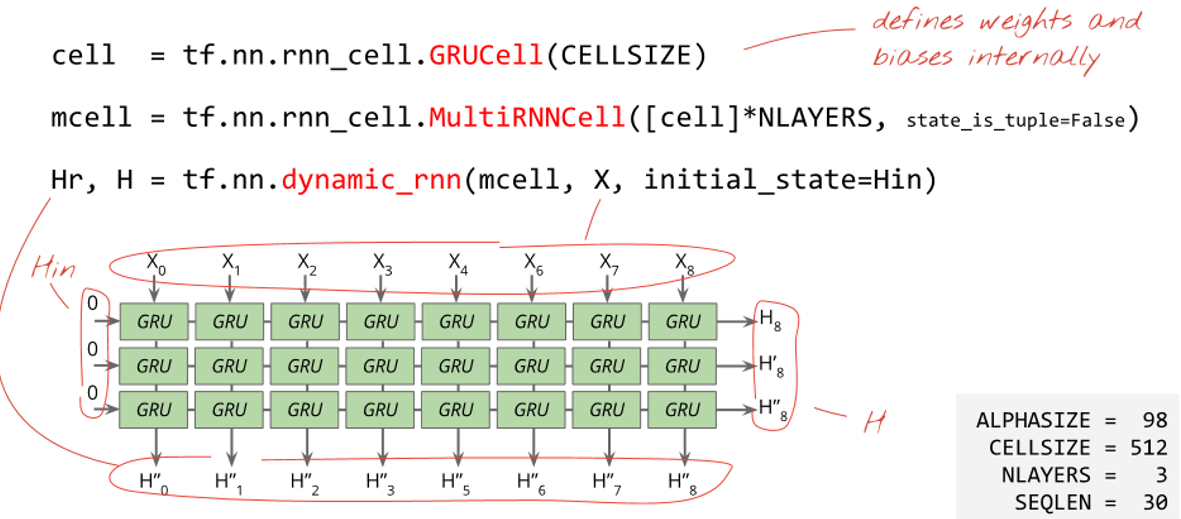
\includegraphics[width=0.8\linewidth,keepaspectratio]{grutf}
\end{center}
\end{frame}


%%%%%%%%%%%%%%%%%%%%%%%%%%%%%%%%%%%%%%%%%%%%%%%%%%%%
%\begin{frame}[fragile] \frametitle{Language model in Tensorflow}
%\begin{center}
%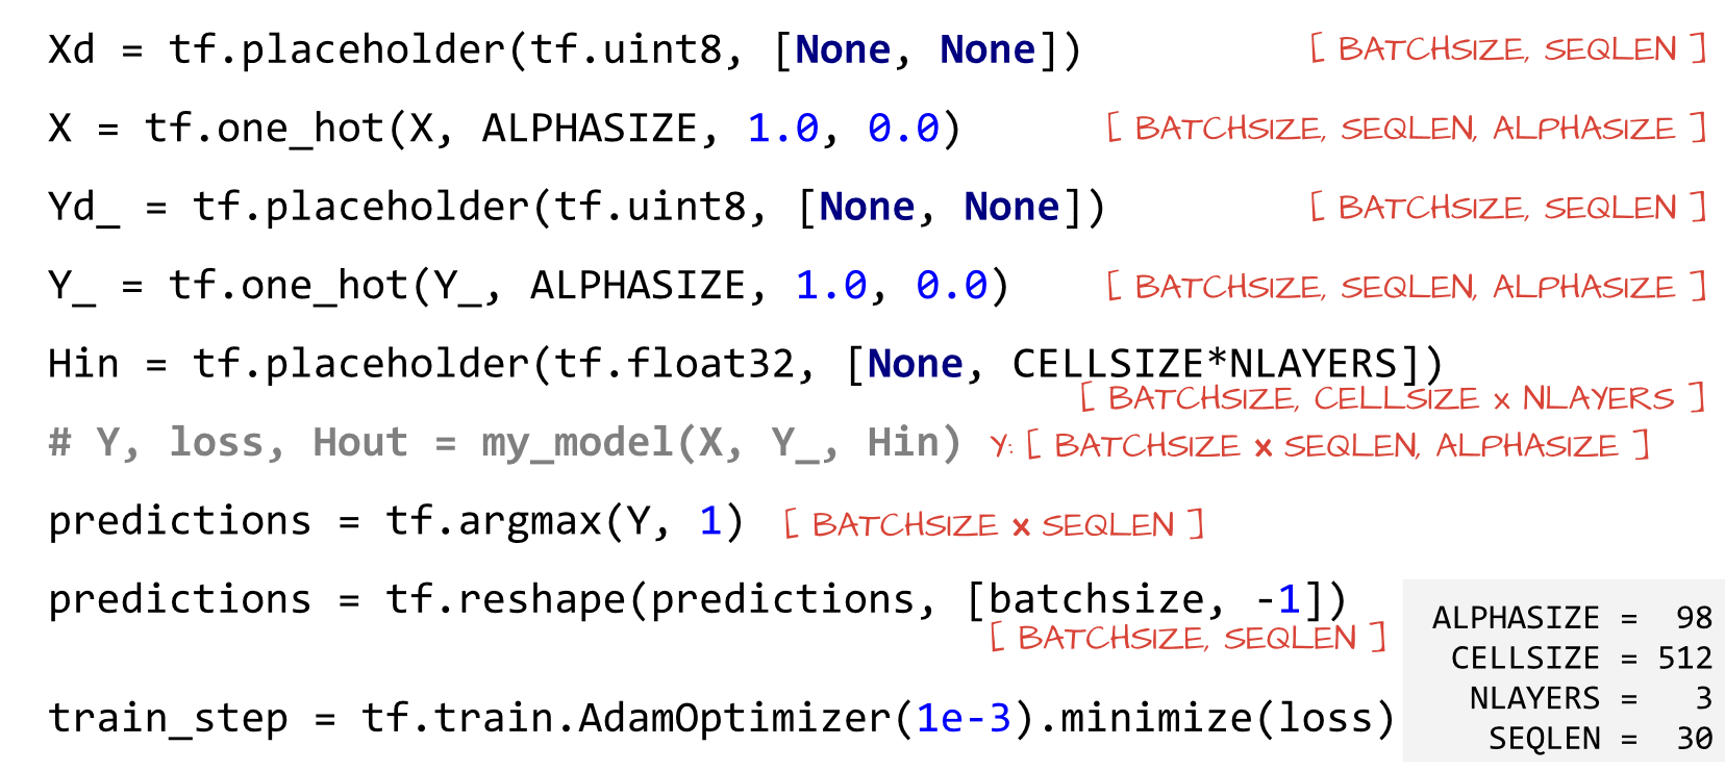
\includegraphics[width=0.8\linewidth,keepaspectratio]{langtf}
%\end{center}
%\end{frame}

%%%%%%%%%%%%%%%%%%%%%%%%%%%%%%%%%%%%%%%%%%%%%%%%%%%%
%\begin{frame}[fragile] \frametitle{Model}
%\begin{center}
%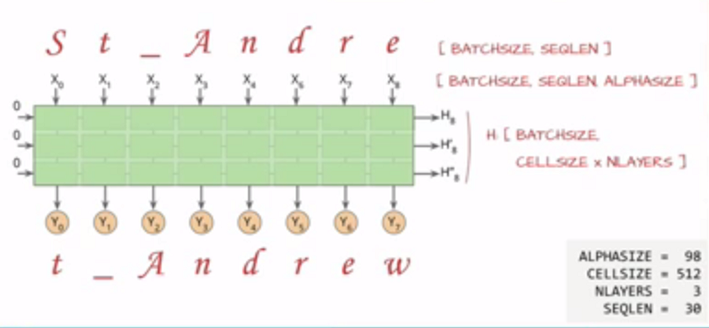
\includegraphics[width=0.8\linewidth,keepaspectratio]{grumodel}
%\end{center}
%\end{frame}

%
%%%%%%%%%%%%%%%%%%%%%%%%%%%%%%%%%%%%%%%%%%%%%%%%%%%%
%\begin{frame}[fragile] \frametitle{Full Code}
%\begin{center}
%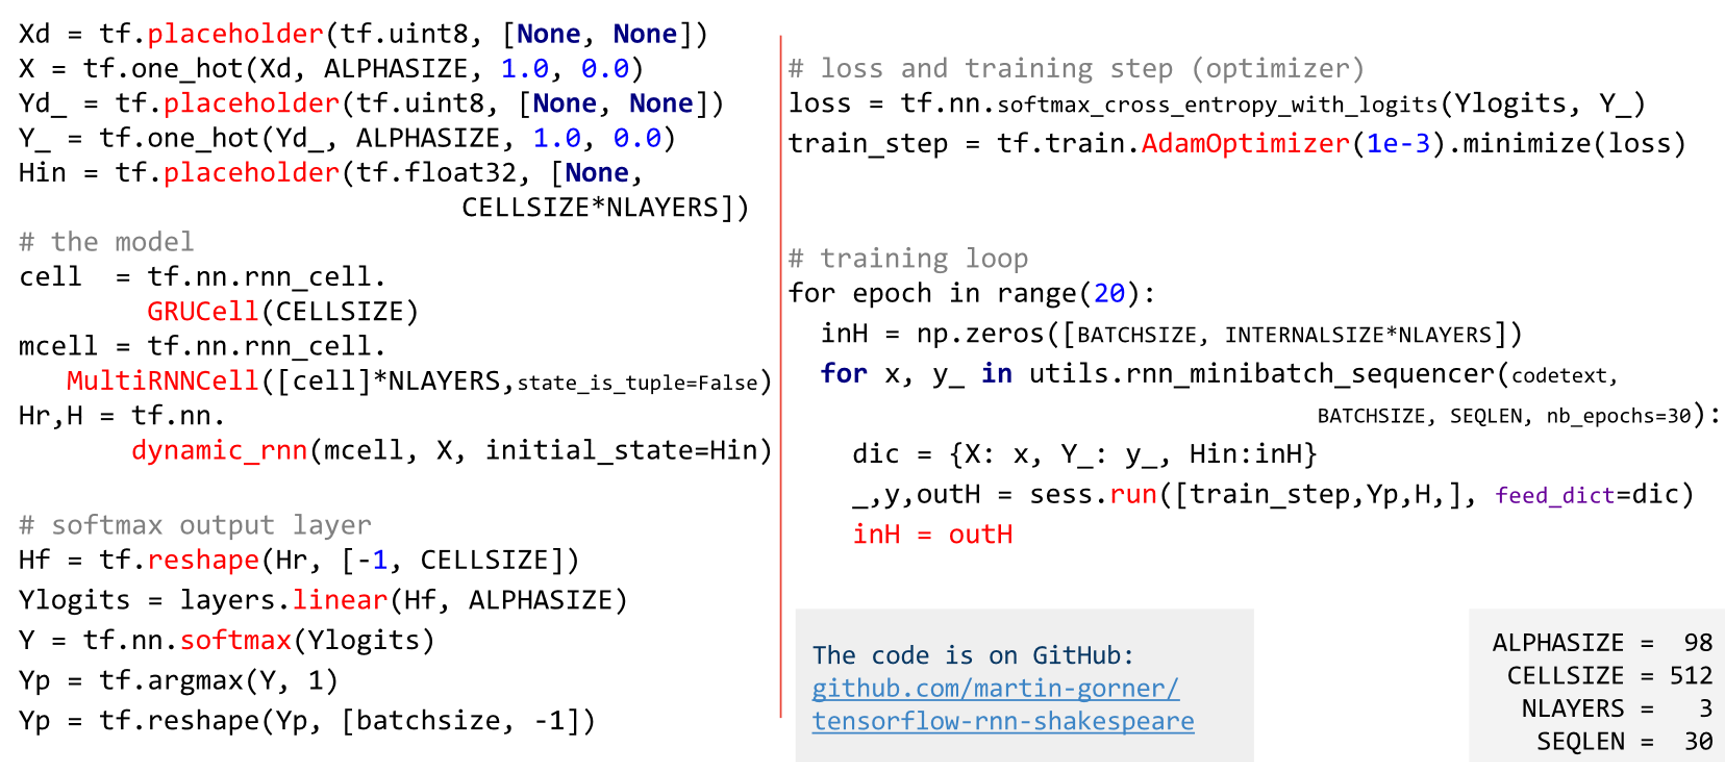
\includegraphics[width=\linewidth,keepaspectratio]{grucode}
%\end{center}
%\end{frame}

%
%%%%%%%%%%%%%%%%%%%%%%%%%%%%%%%%%%%%%%%%%%%%%%%%%%%%
%\begin{frame}[fragile] \frametitle{Applications: Text Classification}
%\begin{center}
%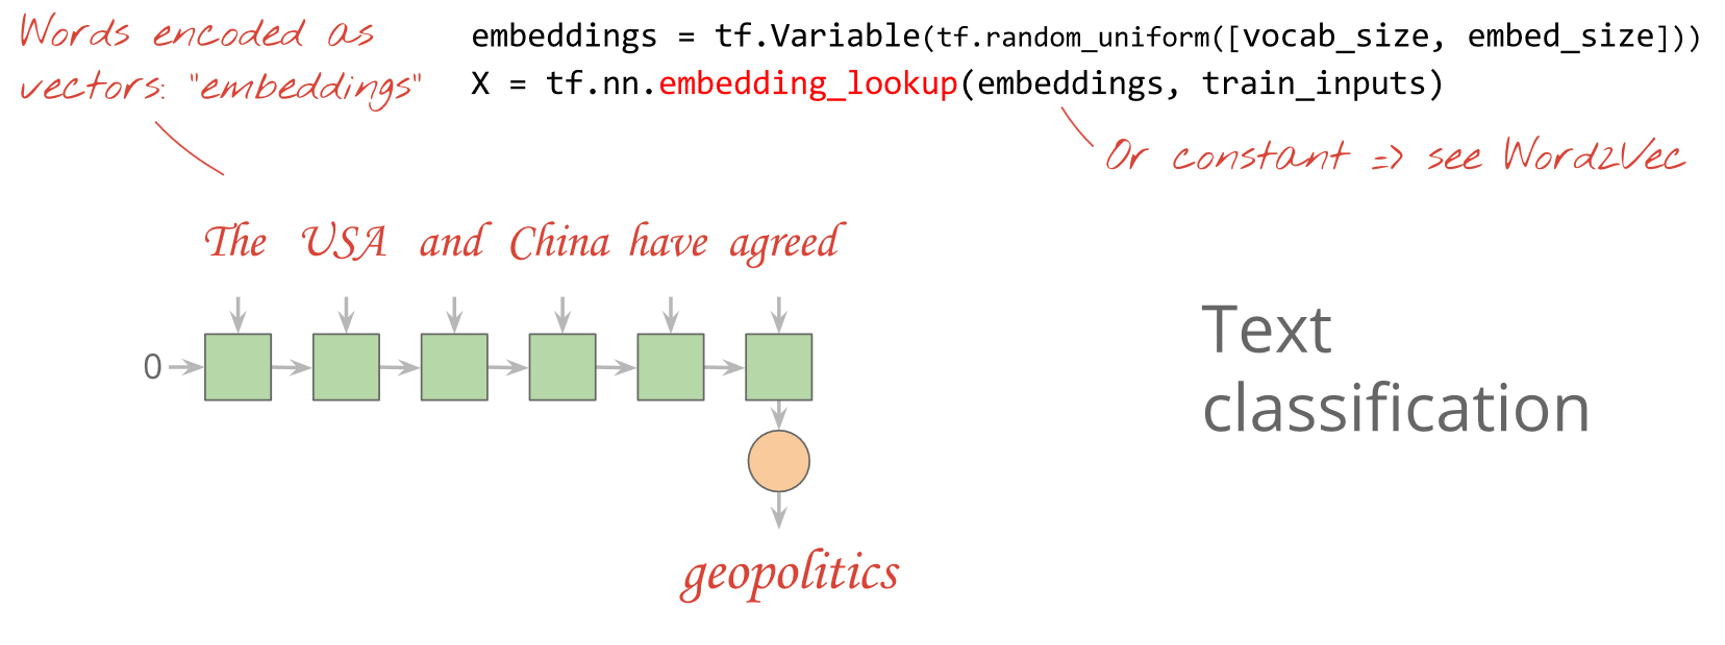
\includegraphics[width=0.8\linewidth,keepaspectratio]{grutext}
%\end{center}
%\end{frame}
%



%%%%%%%%%%%%%%%%%%%%%%%%%%%%%%%%%%%%%%%%%%%%%%%%%%%%
%\begin{frame}[fragile] \frametitle{Convolution Network}
%%
%%\adjustbox{valign=t}{
%%\begin{minipage}{0.45\linewidth}
%\begin{itemize}
%\item Image is input
%\item $W_1$ has window of $5x5$, with channel 1 (mono chrome), wt sets 4
%\item With stride 2, image halved14x14. Previous wt set 4, become input channels now.
%\item Last is fully connected to 10 outputs
%\end{itemize}
%%\end{minipage}
%%}
%%\hfill
%%\adjustbox{valign=t}{
%%\begin{minipage}{0.45\linewidth}
%\begin{center}
%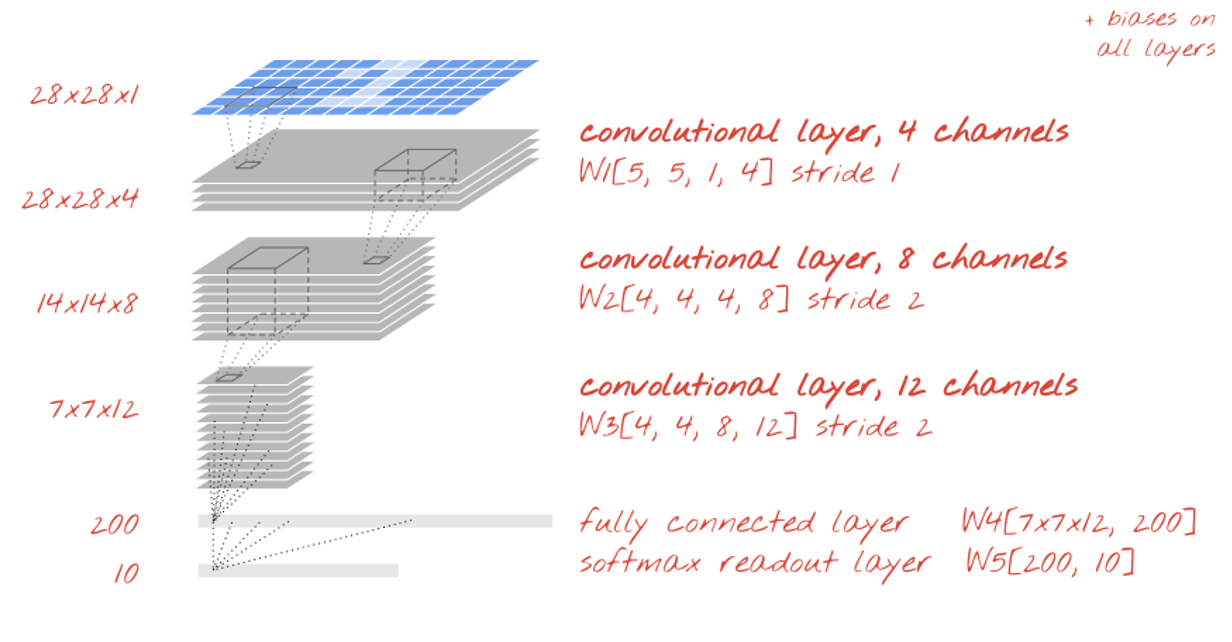
\includegraphics[width=0.8\linewidth,keepaspectratio]{cnnchannel}
%\end{center}
%%\end{minipage}
%%}
%
%\end{frame}
%
%
%%%%%%%%%%%%%%%%%%%%%%%%%%%%%%%%%%%%%%%%%%%%%%%%%%%%
%\begin{frame}[fragile] \frametitle{Convolution layer}
%
%\adjustbox{valign=t}{
%\begin{minipage}{0.45\linewidth}
%\begin{itemize}
%\item Color Images shown as 3 stacks (3 RGB values for each pixel, vertically)
%\item One neuron will be doing weighted sum of X (small patch pixel values)
%\item Next neuron, will take  next patch keeping the weights same.
%\item Once one set of weights is complete, use second set (shown in grey), called output channels
%\end{itemize}
%\end{minipage}
%}
%\hfill
%\adjustbox{valign=t}{
%\begin{minipage}{0.45\linewidth}
%\begin{center}
%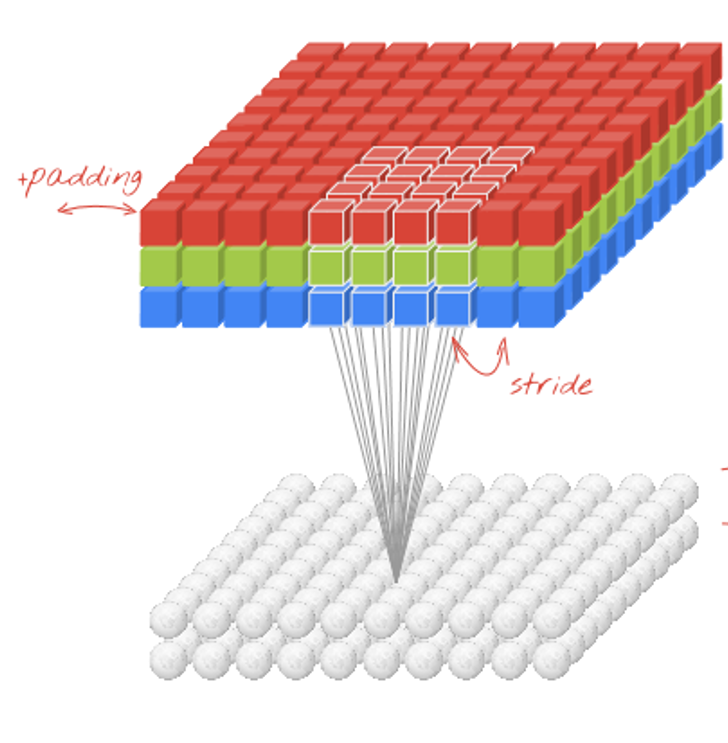
\includegraphics[width=\linewidth,keepaspectratio]{convlayer}
%\end{center}
%\end{minipage}
%}
%
%\end{frame}
%
%
%%%%%%%%%%%%%%%%%%%%%%%%%%%%%%%%%%%%%%%%%%%%%%%%%%%%
%\begin{frame}[fragile] \frametitle{Convolutional Layer Channels}
%
%\begin{center}
%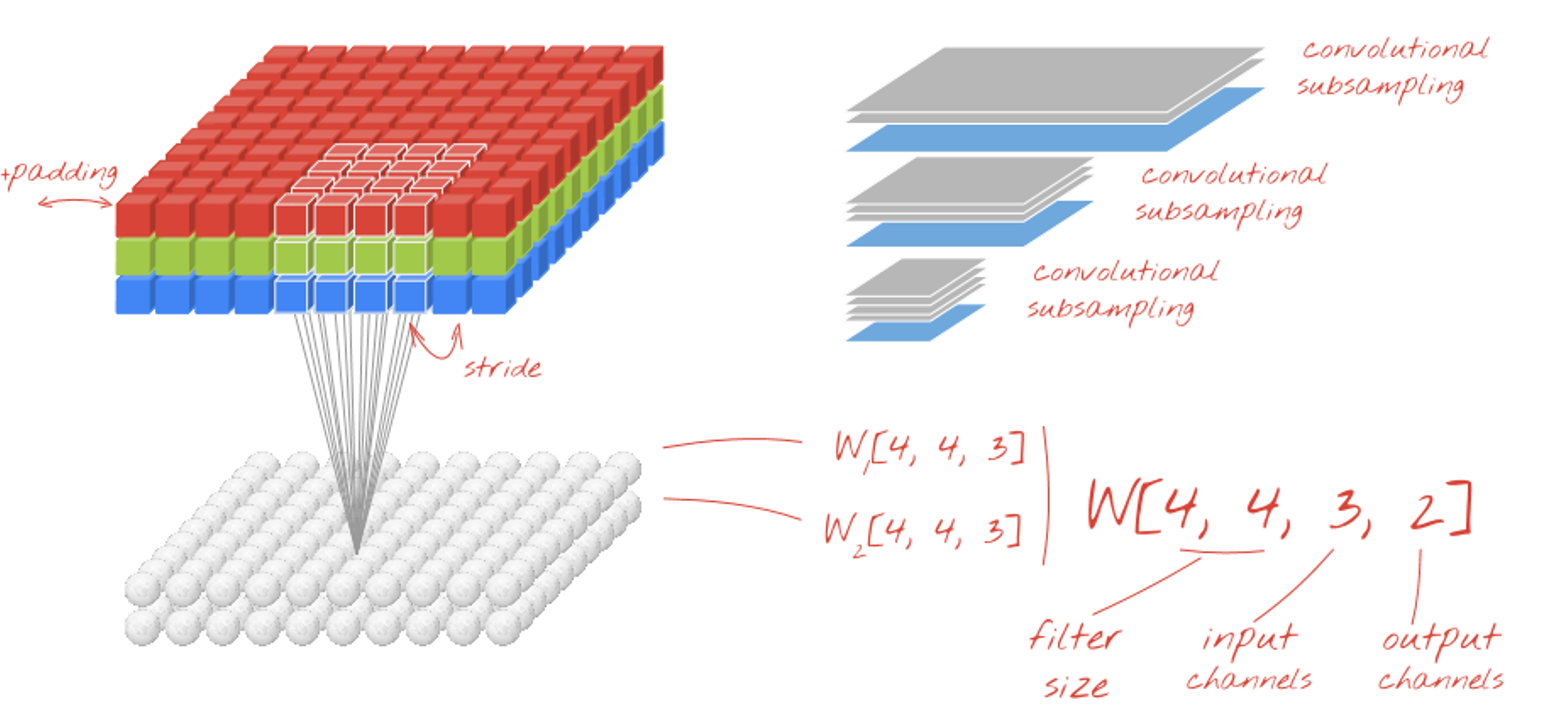
\includegraphics[width=\linewidth,keepaspectratio]{convlayerarray}
%\end{center}
%\end{frame}
%
%%%%%%%%%%%%%%%%%%%%%%%%%%%%%%%%%%%%%%%%%%%%%%%%%%%%
%\begin{frame}[fragile] \frametitle{Convolution parameters}
%
%\adjustbox{valign=t}{
%\begin{minipage}{0.45\linewidth}
%\begin{itemize}
%\item Image window: $4x3$
%\item Channels: 3 (RGB)
%\item Weight sets, output channels: 2
%\begin{itemize}
%\item $W_1 : [4,4,3]$
%\item $W_2: [4,4,3]$
%\item Combined: $W:[4,4,3,2]$
%\end{itemize}
%\item Stride: jumps between window
%\item Padding: extra values at edges
%\end{itemize}
%\end{minipage}
%}
%\hfill
%\adjustbox{valign=t}{
%\begin{minipage}{0.45\linewidth}
%\begin{itemize}
%\item Finally we want 10 outputs (digits). How to bring from so many weights to 10, down?
%\item Subsampling: Takes 4 outputs (2x2), takes max, and passes it to the next layer.
%\item With each layer, image size reduces proportionately
%\end{itemize}
%\end{minipage}
%}
%
%\end{frame}
%
%
%
%%%%%%%%%%%%%%%%%%%%%%%%%%%%%%%%%%%%%%%%%%%%%%%%%%%%
%\begin{frame}[fragile] \frametitle{TensorFlow}
%
%\begin{center}
%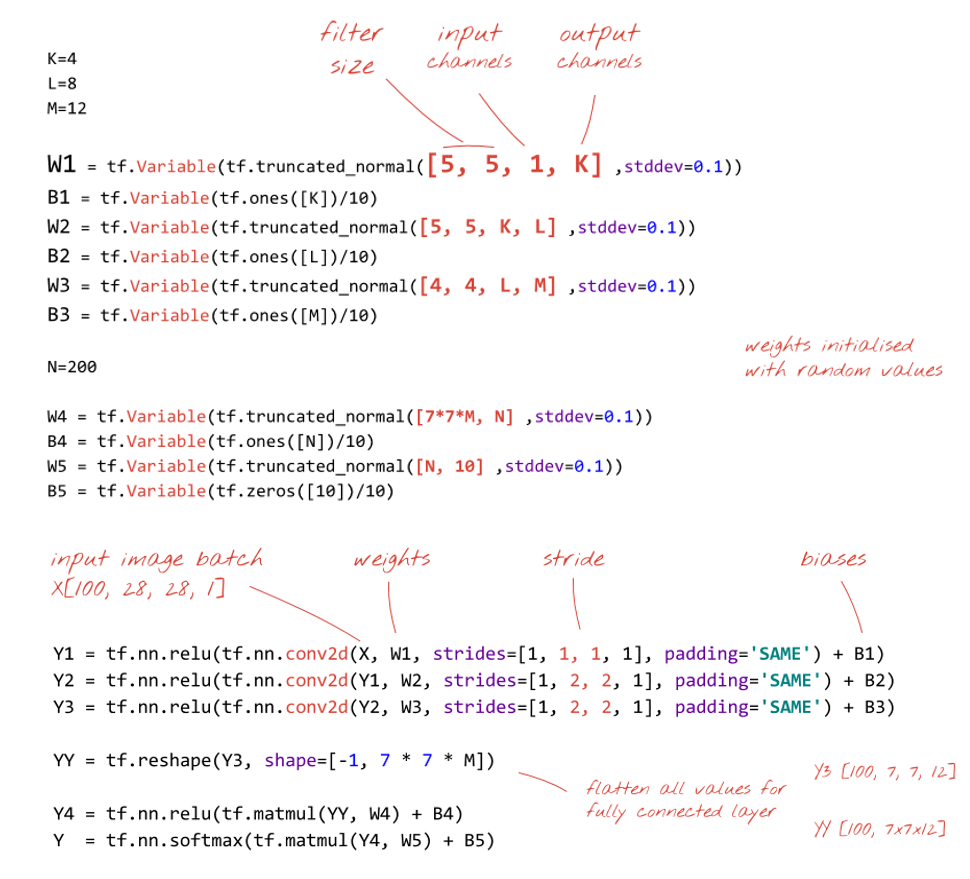
\includegraphics[width=0.7\linewidth,keepaspectratio]{cnntf}
%\end{center}
%
%\end{frame}
%
%
%%%%%%%%%%%%%%%%%%%%%%%%%%%%%%%%%%%%%%%%%%%%%%%%%%%%
%\begin{frame}[fragile] \frametitle{Better network}
%
%99.3\%
%
%\begin{center}
%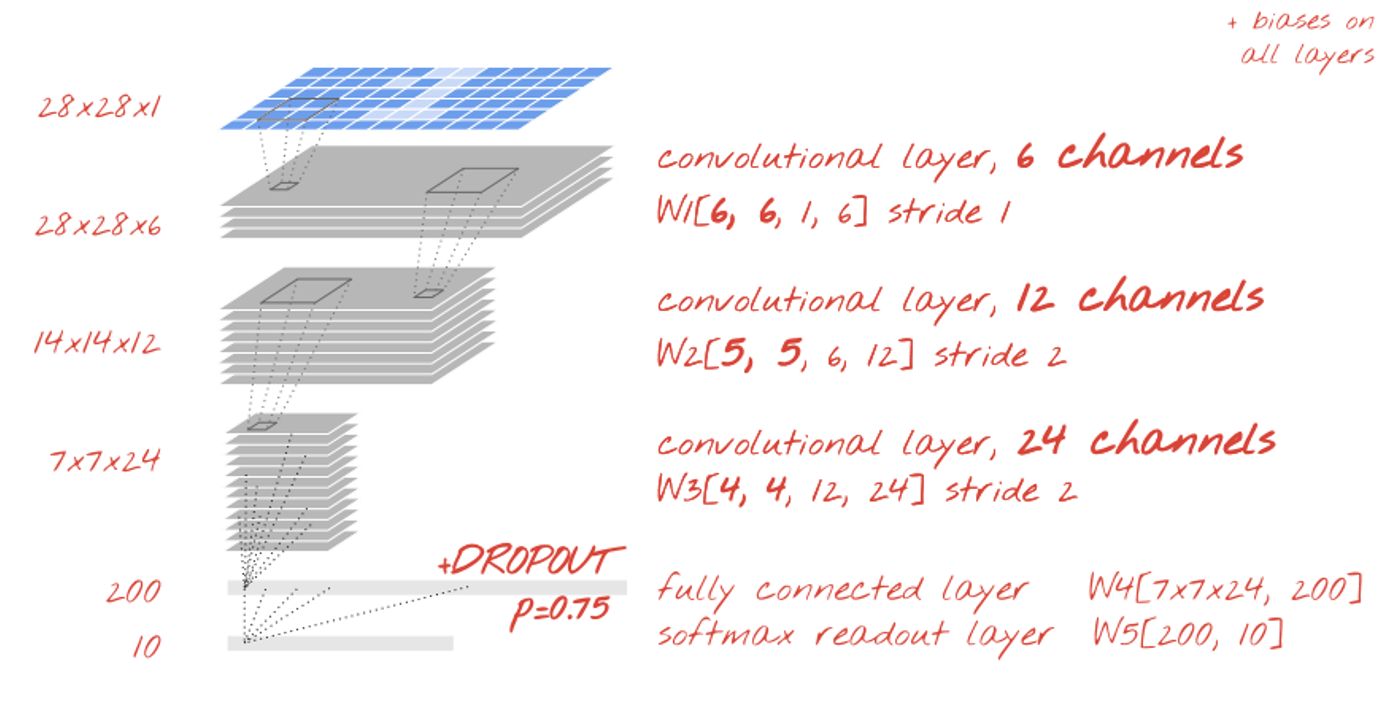
\includegraphics[width=\linewidth,keepaspectratio]{cnnnn}
%\end{center}
%
%\end{frame}
%

